\documentclass[11pt]{article}
\usepackage[margin=1in]{geometry}
\usepackage{graphicx}
\usepackage{microtype}
\usepackage{verbatim}
\usepackage{amsmath}
\usepackage{nicefrac}
\usepackage[colorlinks=false, hidelinks]{hyperref}
\usepackage{caption}
\usepackage{subcaption}
\usepackage{listings}
\usepackage{harmony}
\usepackage{wasysym}

\begin{document}

\title{LFSR and ASG Pseudorandom Number Generators\\Embedded System Design, Lab 5}
\date{October 22, 2015}
\author{Ben Lorenzetti}
\maketitle

\tableofcontents

\clearpage

\section{Objectives and Problem Descriptions}
\subsection{8-Bit Linear Feedback Shift Register (LFSR)}
\label{problem-1-specs}

Implement an 8--bit linear feedback shift register (LFSR) on the PIC16F877 44--Pin Demo Board.
The LFSR should be designed with suitable taps such that 255 unique numbers are produced in a
pseudorandom sequence before the cycle repeats.

The 8--bits should be displayed on the 8 LEDs connected to Port D on the demo board.
The LFSR should cycle (change state) once per second.

\subsection{Alternating Step Generator (ASG)}
\label{problem-2-spces}

Implement an alternating step generator (ASG) on the PIC16F877 44--pin demo board.
The ASG should be comprised of three LFSRs with 14--bit, 15--bit, and 16--bit
lengths. The pseudorandom bit sequence produced by the ASG should be displayed
on the 8 LEDs on board the 44--pin demo board. Eight new bits should be displayed
every second.

The ASG should be implemented with suitable taps such that each LFSR produces the
maximum length sequence for it's bit size. One LFSR should be cycled each iteration,
and the output bit from this LFSR should be used to select one of the other two.
From the other two LFSRs, the register which is cycled produces the output bit
of the ASG for that cycle.

\section{Procedure}
\subsection{Reading Assignments}

The lab procedure and the blackboard post had a cornucopia of reading assignments,
including the user manuals for MPLAB X IDE, the PIC Assembler, the 44--pin demo board,
and online getting started guides.

There was way to much to actually read, but some of it was helpful. Particularly
the first sections of the online getting started with MPLAB guide and the Assembler
Users Manual. The PIC16F877 datasheet was also useful since the PDF is searchable.

\subsection{LFSRs and ASGs Theory}

A linear--feedback shift register (LFSR) is a shift register whose input is a linear,
real time function of its current state.

Usually the linear function is a cascade of XOR gates that ``tap'' some of the upper
order bits on the LFSR. The tapped bits are know as the feedback polynomial for the
LFSR. If the feedback function is constructed as a cascade of XOR gates, the LFSR
is known as a Fibonacci LFSR. An example of a 14--bit Fibonacci LFSR is shown 
in figure \ref{14-bit-fibonacci-with-feedback-polynomial}.

\begin{center}
	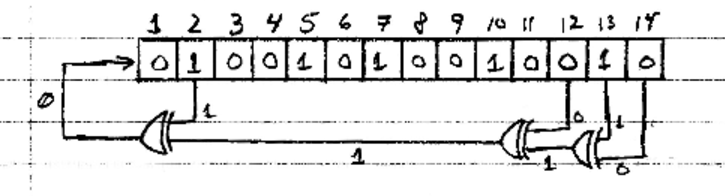
\includegraphics[width=0.7\textwidth]{Figures/14-bit-fibonacci-with-feedback-polynomial.pdf}
	\captionof{figure}{A 14-bit Fibonacci LFSR with feedback polynomial $F(x)=x^{14}+x^{13}+x^{12}+x^{2}+1$}
	\label{14-bit-fibonacci-with-feedback-polynomial}
\end{center}

LFSRs are often used as pseudorandom number generators and the initial value is know
as the ``seed'' value. For Fibonacci LFSRs, a seed value of zero will cause the LFSR
to be forever stuck in the zero state.

If the feedback polynomial is chosen correctly, the LFSR can produce $2^{n}-1$
(not including 0) pseudorandom numbers before the sequence begins to repeat.
It turns out that all of the LFSRs of bit length $n$ with a sequence $2^{n}-1$
long have some similarities. They have an even number of taps and all of the tap
locations, taken together, must be relatively prime. For example, an LFSR tapped
at bits 2 and 4 or 2 and 8 would certainly not have the maximum sequence length.
Some feedback polynomials that are know to produce maximum length sequences are
listed in table \ref{feedback-polynomials-table}.

\begin{table}
\centering
\caption{Feedback Polynomials with Maximum Length Sequences}
\begin{tabular}{c | l | c | c}
\hline\hline
Size of LFSR	&Feedback Polynomial	&Sequence Length	&\texttt{TAP\_MASK}	\\
\hline
3--bits	&$x^{3}+x^{2}+1$		&7	&\texttt{0x0006}	\\
4--bits	&$x^{4}+x^{3}+1$		&15	&\texttt{0x000C}	\\
5--bits	&$x^{5}+x^{3}+1$		&31	&\texttt{0x0014}	\\
6--bits	&$x^{6}+x^{5}+1$		&63	&\texttt{0x0030}	\\
7--bits	&$x^{7}+x^{6}+1$		&127	&\texttt{0x0060}	\\
8--bits	&$x^{8}+x^{6}+x^{5}+x^{4}+1$	&255	&\texttt{0x00D8}	\\
14--bits&$x^{14}+x^{13}+x^{12}+x^{2}+1$	&16383	&\texttt{0x3802}	\\
15--bits&$x^{15}+x^{14}+1$		&32767	&\texttt{0x6000}	\\
16--bits&$x^{16}+x^{14}+x^{13}+x^{11}+1$&65535	&\texttt{0xB400}	\\
\hline\hline
\end{tabular}
\label{feedback-polynomials-table}
\end{table}

\subsection{Implementation Design}

\begin{figure}
	\centering
	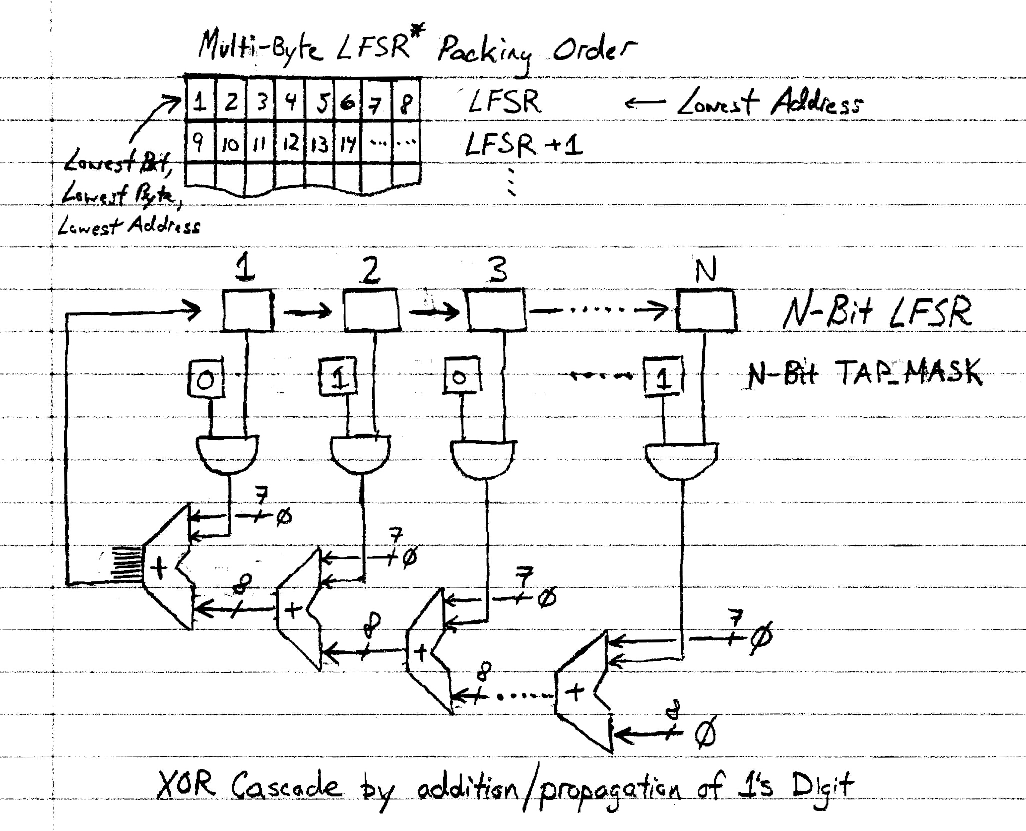
\includegraphics[width=0.75\textwidth]{Figures/fibonacci-equivalent-circuit.pdf}
	\caption{Equivalent Circuit Implementation of an Arbitrary Length Fibonacci LFSR}
	\label{fibonacci-equivalent-circuit}
\end{figure}

Bitwise manipulation is always difficult in any programming language because
computers and microcontrollers are designed to use data in groups of bytes---or
whatever the word size of the machine may be.

Luckily, the PIC instruction set has rotate left and rotate right instructions
which can shift bits in and out of a byte like a queue. Nine bits are involved,
eight bits from the byte being rotated and a ninth bit---the carry flag from
the status register. The \texttt{STATUS, C} flag is set by many ALU operations but, in the case
of rotate left and rotart right, the value in the Carry Flag is shifted into
the byte and is replaced by the value shifting out the other side of the byte queue.
The assembler mnemonics for rotate left and rotate right are:
\begin{verbatim}
  RLF  f, d  ; f is address of the operand value and d is result destination
  RRF  f, d  ; d=1 stores result back at ADDR f, d=0 stores result in W
\end{verbatim}

My design for a generic length LFSR takes takes advantage of these rotate instructions.
The hardware concept for my design is shown in figure \ref{fibonacci-equivalent-circuit}.
This arrangement of hardware lends itself to implementable in software because there are few
conditional statements; the XOR cascade can be implemented as a loop instead of
a unique--per--feedback--polynomial sequence of logic statements. Also, instead of
trying to arrange bits to overlap for \texttt{XOR} operations, it propagates the
XOR signal in the 1's Digit of a register with repeated addition of \texttt{0} or \texttt{1}.
This has an effect equivalent to XORing if you ignore the higher order bits.

\begin{figure}
	\centering
	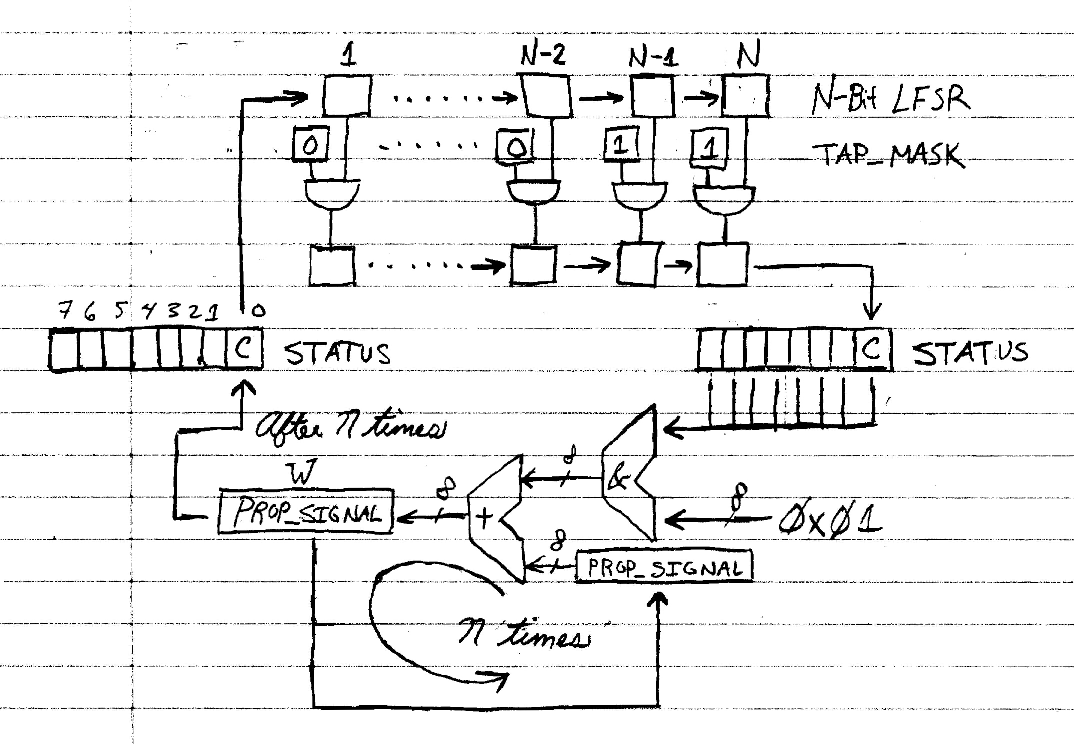
\includegraphics[width=0.75\textwidth]{Figures/xor-propagation-flowchart.pdf}
	\caption{Implementation of XOR Propagation}
	\label{xor-propagation-flowchart}
\end{figure}

Since LFSRs are easily visuallized as hardware, a flowchart for the XOR function
implementation is similarly drawn in figure \ref{xor-propagation-flowchart}.
This flowchart shows the value of the PIC architecture's Carry Flag for implementing an LFSR.

\begin{figure}
	\centering
	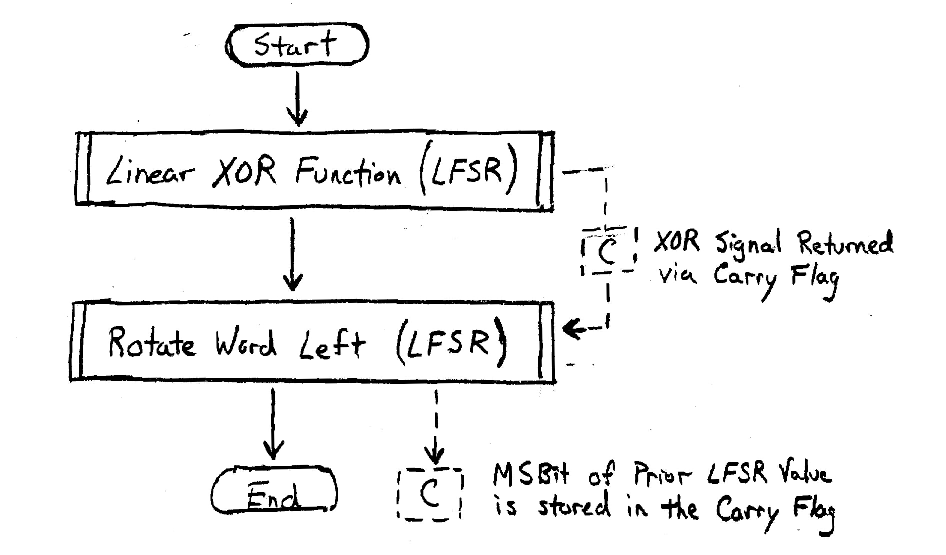
\includegraphics[width=0.6\textwidth]{Figures/cycle-lfsr-flowchart.pdf}
	\caption{Cycle LFSR Function Implementation Flowchart}
	\label{cycle-lfsr-flowchart}
\end{figure}

The full process of advancing to the next state in the LFSR sequence involves
calculating the result of the linear XOR function and then shifting the LFS register
by 1--bit with the XOR result as input. This is shown in the implementation
flowchart in figure \ref{cycle-lfsr-flowchart}.
\subsection{Hello World Program (Delay Function)}

\subsection{Assembly Macros (Rotate Word Function)}

\subsection{XOR Propagation Function}

\subsection{8-Bit LFSR Design}

\begin{figure}
	\centering
	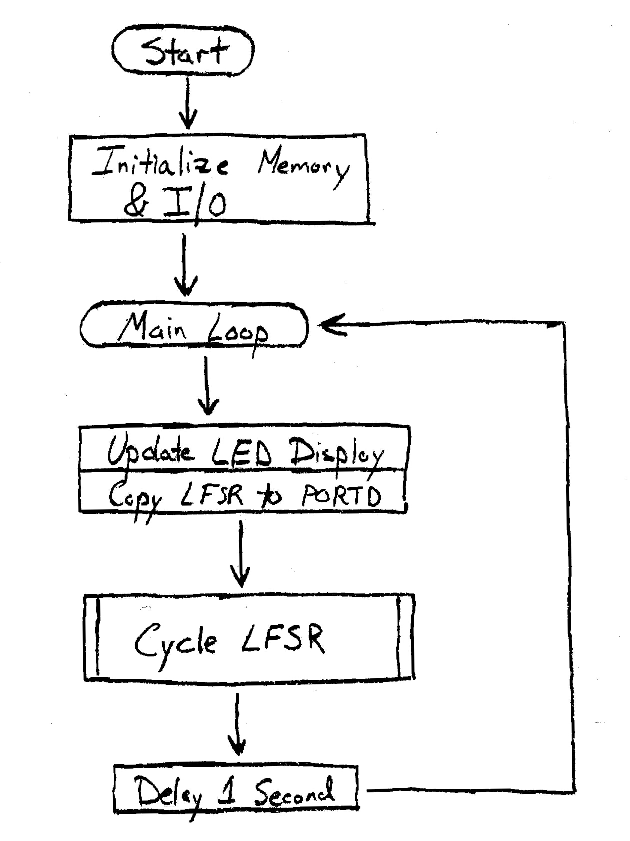
\includegraphics[width=0.35\textwidth]{Figures/8-bit-lfsr-flowchart.pdf}
	\caption{8-Bit LFSR Implementation Flowchart}
	\label{8-bit-lfsr-flowchart}
\end{figure}

\subsection{ASG Design}

\begin{figure}
	\centering
	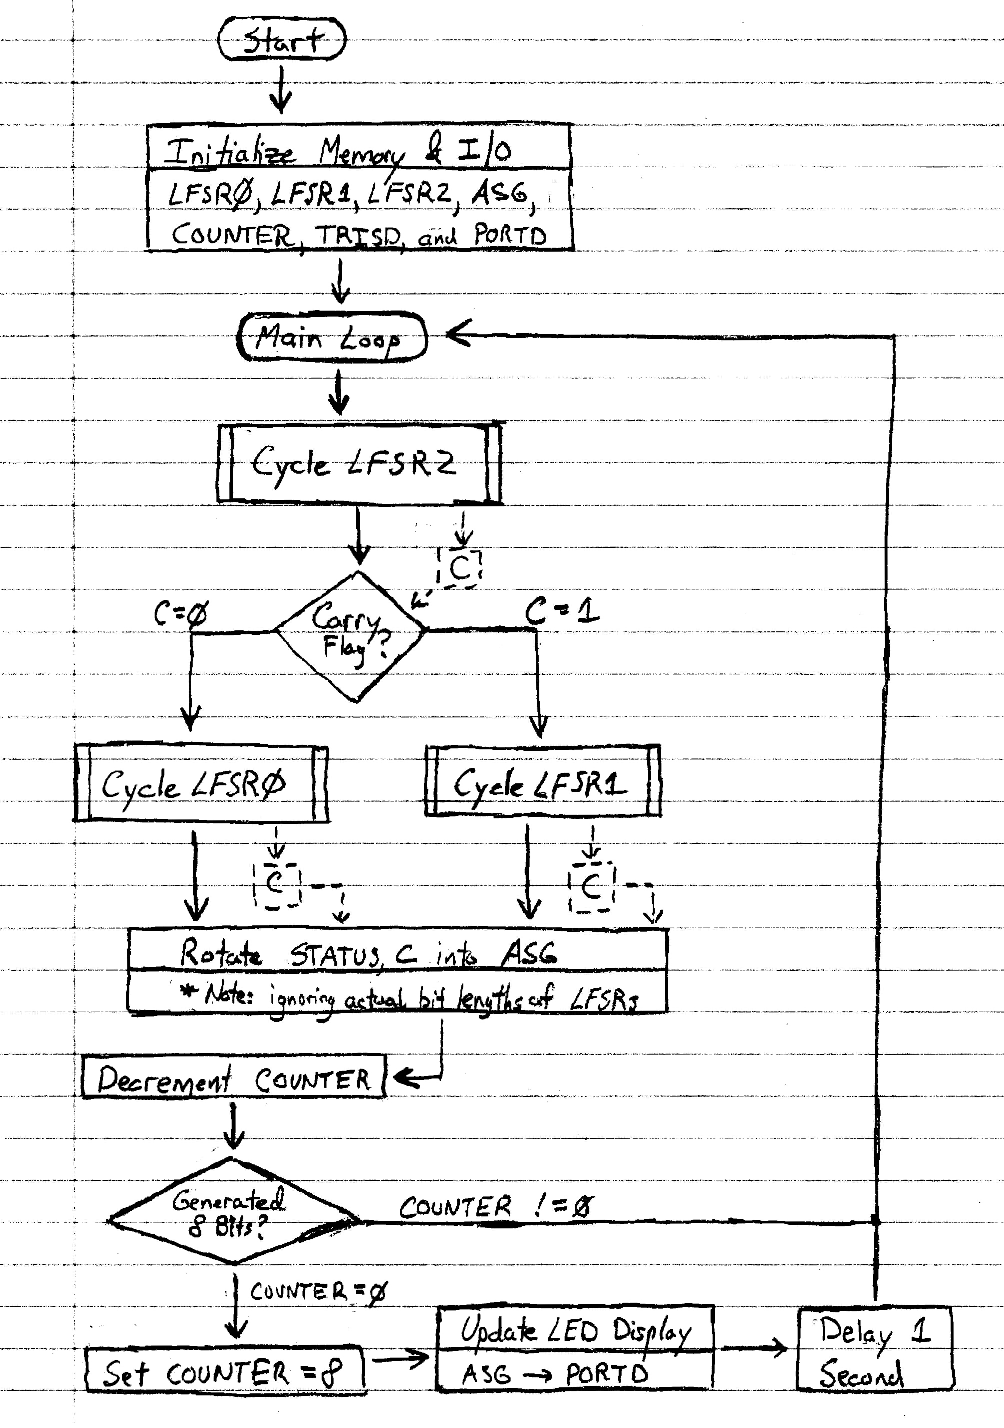
\includegraphics[width=0.6\textwidth]{Figures/alternating-step-generator-flowchart.pdf}
	\caption{Alternating Step Generator Implementation}
	\label{alternating-step-generator-flowchart}
\end{figure}

\section{Expected Results}

\subsection{3-Bit LFSR Demonstration}

\subsection{8-Bit LFSR Demonstration}

\subsection{ASG Demonstration}

\section{Experiment and Design Revisions}

\subsection{Addition of Macros}

\subsection{Use of Carry Flag between Functional Blocks}

\section{Observations}

\subsection{Observations}

\section{Discussion}

\subsection{Discussion of Results}

\subsection{Carry Flag and PIC Design}

\section{Exercises}

\clearpage
\section{Implementation Code}

\subsection{8-Bit LFSR}
\label{lsfr-code}

\lstinputlisting[breaklines]{Eight-Bit-LFSR/lfsr.asm}


\clearpage
\subsection{Alternating Step Generator}
\label{asg-code}

\lstinputlisting[breaklines]{Alternating-Step-Generator/asg.asm}



\end{document}
